\documentclass[letterpaper,11pt]{memoir}
  \usepackage[utf8]{inputenc}
  \usepackage{fourier,microtype}       % texte en Utopia
  \usepackage[scaled=0.82]{beramono}   % code en Bera
  \renewcommand{\sfdefault}{Myriad-LF} % titres en MyriadPro
  \usepackage{natbib,url}
  \usepackage[english,francais]{babel}
  \usepackage[autolanguage]{numprint}
  \usepackage{vgmath,actu,amsmath,amsthm,amsfonts,icomma}
  \usepackage[noae]{Sweave}
  \usepackage{paralist}
  \usepackage[shortlabels]{enumitem}
  \usepackage{textpos}
  \usepackage{graphicx,color,soulutf8}
  \usepackage{MnSymbol,applekeys}      % symboles spéciaux
  \usepackage{expdlist}
  \usepackage{listingsutf8,answers}
  \usepackage{pdfpages}                % couvertures
  \usepackage{xr}                      % références au chap. 6

  %%% Références externes
  \externaldocument{avance}

  %%%  Couleurs
  \definecolor{comments}{rgb}{0.7,0,0}
  \definecolor{darkred}{rgb}{0.8,0,0}
  \definecolor{shadecolor}{gray}{0}
  \definecolor{link}{rgb}{0,0,0.4}
  \definecolor{videotag}{rgb}{0,0,0.75}

  %%% Hyperliens
  \usepackage{hyperref}
  \hypersetup{colorlinks,allcolors=link}

  %%% ============
  %%%  Page titre
  %%% ============
  \title{%
    \fontseries{b}\fontsize{42}{33}\selectfont ACT 2002 \\
    \fontseries{m}\fontsize{32}{33}\selectfont Méthodes numériques \\
                                               en actuariat \\[20mm]
    \fontseries{b}\fontsize{36}{36}\selectfont Partie II \\
    \fontseries{m}\fontsize{32}{36}\selectfont Simulation stochastique}
  \author{%
    \fontseries{b}\fontsize{16}{20}\selectfont Vincent Goulet \\
    \fontseries{m}\fontsize{14}{18}\selectfont Professeur titulaire \textbar\
                                               École d'actuariat \textbar\
                                               Université Laval}
  \date{%
    \fontseries{m}\fontsize{14}{18}\selectfont Notes de cours \textbar\
                                               Exercices \textemdash\
                                               édition 2013}

  %%% ===================
  %%%  STYLE DU DOCUMENT
  %%% ===================

  %% Titres des chapitres
  \chapterstyle{hangnum}
  \renewcommand{\chaptitlefont}{\normalfont\Huge\sffamily\bfseries\raggedright}

  %% Marges, entêtes et pieds de page
  \setlength{\marginparsep}{7mm}
  \setlength{\marginparwidth}{13mm}
  \setlength{\headwidth}{\textwidth}
  \addtolength{\headwidth}{\marginparsep}
  \addtolength{\headwidth}{\marginparwidth}

  %% Titres des sections et sous-sections
  \setsecheadstyle{\normalfont\Large\sffamily\bfseries\raggedright}
  \setsubsecheadstyle{\normalfont\large\sffamily\bfseries\raggedright}
  \maxsecnumdepth{subsection}
  \setsecnumdepth{subsection}

  %% Listes. Paramétrage avec enumitem.
  \setenumerate{leftmargin=*,align=left}
  \setenumerate[2]{label=\alph*)}
  \setenumerate[3]{label=\roman*),align=right}
  \setitemize{leftmargin=*,align=left}

  %% Noms de fonctions, code, etc.
  \newcommand{\code}[1]{\texttt{#1}}
  \newcommand{\pkg}[1]{\textbf{#1}}

  %% Environnements d'exemples et al.
  \theoremstyle{plain}
  \newtheorem{thm}{Théorème}[chapter]

  \theoremstyle{definition}
  \newtheorem{exemple}{Exemple}[chapter]
  \newtheorem{definition}{Définition}[chapter]
  \newtheorem*{astuce}{Astuce}

  \theoremstyle{remark}
  \newtheorem*{remarque}{Remarque}
  \newtheorem*{remarques}{Remarques}
  \newenvironment{rem}{\begin{remarque} \mbox{}}{\end{remarque}}
  \newenvironment{rems}{\begin{remarques} \mbox{}}{\end{remarques}}

  %% Options de babel
  \frenchbsetup{CompactItemize=false,%
    ThinSpaceInFrenchNumbers=true,
    ItemLabeli=$\filledtriangleright$,
    ItemLabelii=\textendash}
  \addto\captionsfrench{\def\figurename{{\scshape Fig.}}}
  \addto\captionsfrench{\def\tablename{{\scshape Tab.}}}

  %%% =========================
  %%%  Nouveaux environnements
  %%% =========================

  %% Listes d'objectifs au début des chapitres
  \newenvironment{objectifs}{%
    \noindent
    \begin{framed}
      \vspace{-1.33\baselineskip}
      \begin{shaded}
        \noindent\sffamily\bfseries\textcolor{white}{Objectifs du chapitre}
      \end{shaded}
      \vspace{-0.6\baselineskip}
      \setlength{\labelsep}{1ex}
      \settowidth{\labelwidth}{$\filledtriangleright$}
      \setlength{\leftmargini}{\labelwidth}
      \addtolength{\leftmargini}{\labelsep}
      \begin{compactitem}
        \small}
      {\end{compactitem}
    \end{framed}}

  %% Environnements de Sweave
  \DefineVerbatimEnvironment{Sinput}{Verbatim}{xleftmargin=\parindent}
  \DefineVerbatimEnvironment{Soutput}{Verbatim}{xleftmargin=\parindent}
  \DefineVerbatimEnvironment{Scode}{Verbatim}{xleftmargin=\parindent}
  \fvset{listparameters={\setlength{\topsep}{0pt}}}
  \renewenvironment{Schunk}{\vspace{\topsep}}{\vspace{\topsep}}

  %% Exercices et réponses
  \Newassociation{sol}{solution}{solutions}
  \Newassociation{rep}{reponse}{reponses}
  \newcounter{exercice}[chapter]
  \newenvironment{exercice}{%
    \begin{list}{\bfseries \thechapter.\arabic{exercice}}{%
        \refstepcounter{exercice}
        \settowidth{\labelwidth}{\bfseries \thechapter.\arabic{exercice}}
        \setlength{\leftmargin}{\labelwidth}
        \addtolength{\leftmargin}{\labelsep}
        \setdefaultenum{a)}{i)}{}{}}\item}
    {\end{list}}
  \renewenvironment{reponse}[1]{%
    \begin{enumerate}[label=#1,font=\bfseries]
      \setenumerate[2]{leftmargin=*,labelsep=0em}
    \item}
    {\end{enumerate}}
  \renewcommand{\reponseparams}{{\thechapter.\theexercice}}
  \renewenvironment{solution}[1]{%
    \begin{enumerate}[label=#1,font=\bfseries]
      \setenumerate[2]{leftmargin=*,labelsep=0em}
      \item}
    {\end{enumerate}}
  \renewcommand{\solutionparams}{{\thechapter.\theexercice}}

  %%% Changements au fil de la lecture
  \newenvironment{gotoR}{%
    \begin{framed}%
      \noindent
      \begin{minipage}{0.07\linewidth}
        \raisebox{-0.5em}[0em][0em]{\LARGE\color{darkred}\noway}
      \end{minipage}
      \begin{minipage}[t]{0.88\linewidth}}
      {\end{minipage}%
    \end{framed}}

  %%% =============================================
  %%%  Paramètres pour les sections de code source
  %%% =============================================
  \lstloadlanguages{R}
  \lstset{language=R,
    extendedchars=true,
    inputencoding=utf8/latin1,
    basicstyle=\small\ttfamily,
    commentstyle=\color{comments}\slshape,
    keywordstyle=\mdseries,
    showstringspaces=false}

  %%% =====================
  %%%  Nouvelles commandes
  %%% =====================
  \newcommand{\R}{\mathbb{R}}
  \newcommand{\Fonction}[1]{\code{#1}}
  \newcommand{\fonction}[1]{\code{#1}}
  \newcommand{\argument}[1]{\code{#1}}

  %%% Indications de capsule vidéo
  \setulcolor{videotag}
  \setul{1.5pt}{0.7pt}
  \newcommand{\video}{%
    $\mathrel{\vcenter{\offinterlineskip%
        \color{videotag}
        \fontsize{32}{32}\selectfont
        \hbox{$\bigcirc$}%
        \fontsize{24}{22}\selectfont\vskip-21.5pt\hskip5pt
        \hbox{$\filledmedtriangleright$}}}$}
  \newcommand{\capsule}[1]{\marginpar{\video}\ul{#1}}


  %%% Aide pour la césure
  \hyphenation{con-gru-en-tiels}

  %%% Style de la bibliographie
  \bibliographystyle{francais}

  %%% Numérotation des chapitres
  \setcounter{chapter}{6}

%  \includeonly{generation}

\begin{document}

\frontmatter

\pagestyle{empty}
%% Page couverture avant. Il faut modifier la largeur des graphiques
%% puisque Sweave la règle à 0.8\textwidth.
\setkeys{Gin}{width=\paperwidth}
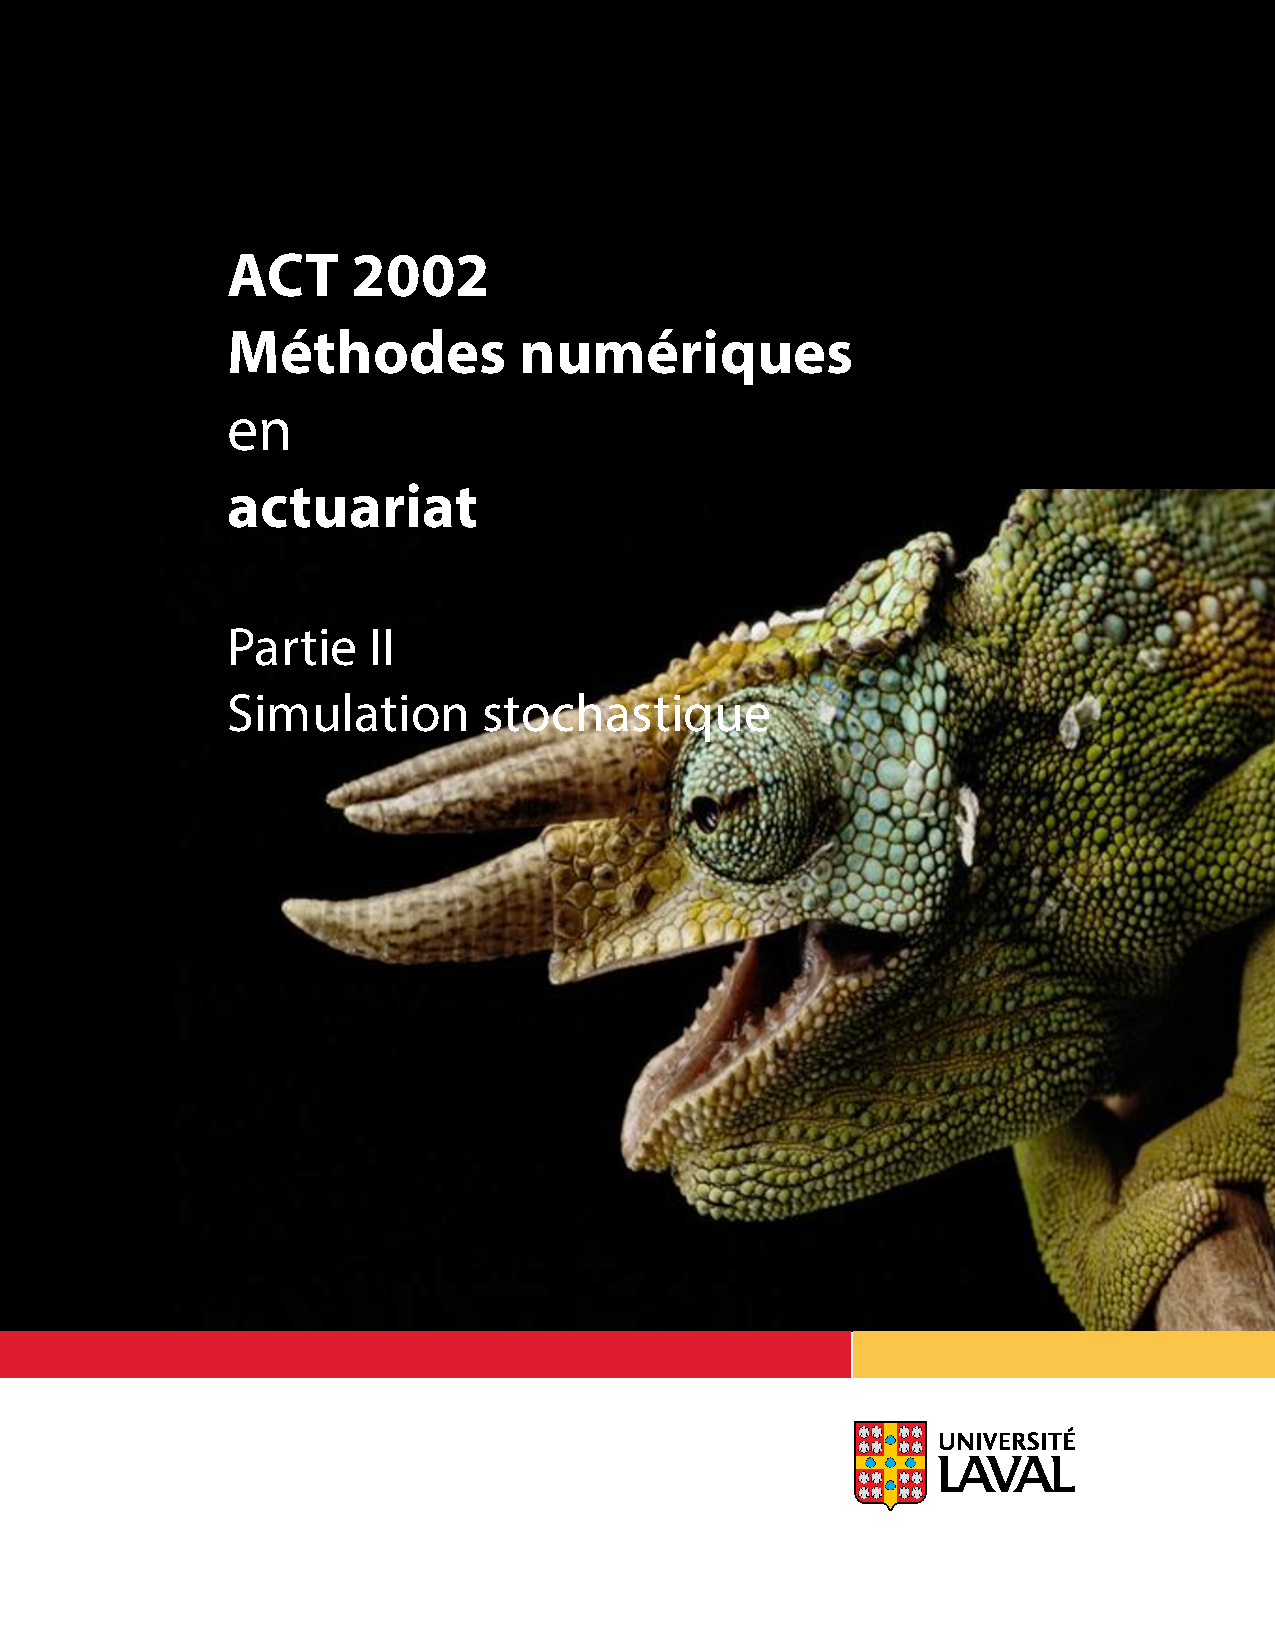
\includepdf[pages=1]{couvertures-partie_2}
\setkeys{Gin}{width=0.8\textwidth}
\cleardoublepage

\begin{adjustwidth*}{-12mm}{-72mm}
  \sffamily
  \raggedright
  \vspace*{-17mm}
  \thetitle \\
  \vspace*{20mm}
  \theparttitle \\
  \vspace*{32mm}
  \theauthor \\
  \vspace*{\fill}
  \thedate
\end{adjustwidth*}

%%% Local Variables:
%%% mode: latex
%%% TeX-master: "methodes_numeriques-partie_3"
%%% coding: utf-8
%%% End:

\clearpage

\begingroup
\calccentering{\unitlength}
\begin{adjustwidth*}{\unitlength}{-\unitlength}
  \setlength{\parindent}{0pt}
  \setlength{\parskip}{\baselineskip}

  {\textcopyright} {\year} Vincent Goulet \\

  
\includegraphics[height=7mm,keepaspectratio=true]{../share/by-sa}\\%
Cette création est mise à disposition selon le contrat
\href{http://creativecommons.org/licenses/by-sa/4.0/deed.fr}{%
  Attribution-Partage dans les mêmes conditions 4.0 International} de
Creative Commons. En vertu de ce contrat, vous êtes libre de:
\begin{itemize}
\item \textbf{partager} --- reproduire, distribuer et communiquer
  l'{\oe}uvre;
\item \textbf{remixer} --- adapter l'{\oe}uvre;
\item utiliser cette {\oe}uvre à des fins commerciales.
\end{itemize}
Selon les conditions suivantes:

\begin{tabularx}{\linewidth}{@{}lX@{}}
  \raisebox{-9mm}[0mm][13mm]{%
    
\includegraphics[height=11mm,keepaspectratio=true]{../share/by}} &
  \textbf{Attribution} --- Vous devez créditer l'{\oe}uvre, intégrer
  un lien vers le contrat et indiquer si des modifications ont été
  effectuées à l'{\oe}uvre. Vous devez indiquer ces informations par
  tous les moyens possibles, mais vous ne pouvez suggérer que
  l'Offrant vous soutient ou soutient la façon dont vous avez utilisé
  son {\oe}uvre. \\
  \raisebox{-9mm}{
\includegraphics[height=11mm,keepaspectratio=true]{../share/sa}}
  & \textbf{Partage dans les mêmes conditions} --- Dans le cas où vous
  modifiez, transformez ou créez à partir du matériel composant
  l'{\oe}uvre originale, vous devez diffuser l'{\oe}uvre modifiée dans
  les même conditions, c'est à dire avec le même contrat avec lequel
  l'{\oe}uvre originale a été diffusée.
\end{tabularx}


  \textbf{Code source} \\
  Le code source {\LaTeX} et R de ce document est disponible à l'adresse
    \url{https://svn.fsg.ulaval.ca/svn-pub/vgoulet/documents/methodes_numeriques/}
  ou en communiquant directement avec l'auteur.

  \textbf{Couverture} \\
  Le reptile en couverture est un caméléon tapis (\emph{Furcifer
    lateralis}) originaire de Madagascar. Adulte, sa taille atteint
  les 25~cm, queue comprise.

  Crédit photo: Michabln Schwarz; \url{http://fc-foto.de/2077174}
\end{adjustwidth*}
\endgroup

%%% Local Variables:
%%% mode: latex
%%% TeX-master: "methodes_numeriques-partie_4"
%%% coding: utf-8
%%% End:

\clearpage

\pagestyle{companion}

\chapter*{Introduction}
\addcontentsline{toc}{chapter}{Introduction}
\markboth{Introduction}{Introduction}

La simulation stochastique est une technique utilisée dans un grand
nombre de domaines. On n'a qu'à penser aux simulations boursières qui
font l'objet d'un concours annuel, aux voitures qui sont d'abord
conçues sur ordinateur et soumises à des tests de collision virtuels,
ou encore aux prévisions météo quid ne en fait les résultats de
simulations de systèmes climatiques d'une grande complexité.

Toute simulation stochastique repose d'abord et avant tout sur une
source de nombres aléatoires de qualité. Comment en générer un grand
nombre rapidement et, surtout, comment s'assurer que les nombres
produits sont bien aléatoires? C'est un sujet d'une grande importance,
mais également fort complexe. Aussi ne ferons-nous que l'effleurer en
étudiant les techniques de base dans le
chapitre~\ref{chap:generation}.

En actuariat, nous avons habituellement besoin de nombres aléatoires
provenant d'une loi de probabilité non uniforme. Le
chapitre~\ref{chap:simulation} présente quelques algorithmes pour
transformer des nombres aléatoires uniformes en nombres non uniformes.
Évidemment, des outils informatiques sont aujourd'hui disponibles pour
générer facilement et rapidement des nombres aléatoires de diverses
lois de probabilité. Nous passons en revue les fonctionnalités de R et
de Excel à ce chapitre.

Enfin, cette partie du cours se termine au
chapitre~\ref{chap:montecarlo} par une application à première vue
inusitée de la simulation, soit le calcul d'intégrales définies par la
méthode dite Monte Carlo.

L'étude de ce document implique quelques allers-retours entre le texte
et les sections de code informatique présentes dans chaque chapitre.
Les sauts vers ces sections sont clairement indiqués dans le texte par
des mentions mises en évidence par le symbole {\ForwardToEnd}.

Un symbole de lecture vidéo dans la marge, tel que ci-contre, indique
qu'une capsule vidéo sur \capsule{le sujet} identifié par la marque de
soulignement est disponible dans le site du cours.

Chaque chapitre comporte des d'exercices. Les réponses de ceux-ci se
trouvent à la fin de chacun des chapitres et les solutions complètes
en annexe.

On trouvera également en annexe un bref exposé sur la planification
d'une simulation en R et des rappels sur la notion de transformation
de variables aléatoire.

Je tiens à souligner la précieuse collaboration de MM.~Mathieu
Boudreault, Sébastien Auclair et Louis-Philippe Pouliot lors de la
rédaction des exercices et des solutions.

%%% Local Variables:
%%% mode: latex
%%% TeX-master: "methodes_numeriques-partie_2"
%%% End:

\cleartorecto
\tableofcontents*

\mainmatter

%% Vignette tirée de xkcd.com
\pagestyle{empty}
\begin{vplace}[0.45]
  \centering
  \setkeys{Gin}{width=\textwidth}
  \begin{minipage}{400pt}
    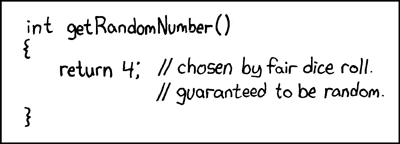
\includegraphics{xkcd.png} \\
    \footnotesize\sffamily%
    Tiré de \href{http://xkcd.com/221/}{XKCD.com}
  \end{minipage}
  \setkeys{Gin}{width=0.8\textwidth}
\end{vplace}
\cleardoublepage

\pagestyle{companion}

\chapter{Génération de nombres aléatoires uniformes}
\label{chap:generation}

\begin{objectifs}
\item Connaître les caractéristiques d'un bon générateur de nombre
  pseudo-aléatoires.
\item Comprendre l'opérateur mathématique modulo.
\item Savoir générer des nombres pseudo-aléatoires à l'aide d'un
  générateur congruentiel linéaire.
\item Savoir établir les caractéristiques d'un générateur congruentiel
  linéaire, notamment sa période.
\item Savoir utiliser les générateurs de nombres aléatoires de Excel,
  VBA et R.
\end{objectifs}

Ce chapitre traite de la simulation de nombres (pseudo) aléatoires
distribués uniformément sur l'intervalle $(0, 1)$. La transformation
de ces nombres uniformes en nombres provenant d'autres distributions
statistiques fera l'objet du prochain chapitre.


\section{Pourquoi faire de la simulation?}
\label{sec:generation:pourquoi}

La simulation stochastique est une technique de plus en plus utilisée
en actuariat comme dans la plupart des sciences appliquées, en génie,
en finance, etc. Les modèles mathématiques et la simulation
stochastiques comportent plusieurs avantages par rapport à
l'expérimentation directe, dont, entre autres:
\begin{itemize}
\item la simulation est non destructrice et peu coûteuse;
\item le système considéré n'a pas besoin d'exister;
\item la simulation est facile à répéter;
\item l'évolution dans la simulation peut être plus rapide que dans la
  réalité;
\item la simulation permet de considérer des modèles très complexes
  impossibles à traiter analytiquement.
\end{itemize}
En revanche, au rayon des inconvénients, on note:
\begin{itemize}
\item le coût (en temps et en argent) de modélisation et de
  programmation s'avère parfois important;
\item le temps d'exécution peut devenir excessif;
\item la simulation ne fournit que des estimations;
\item l'analyse statistique des résultats peut ne pas toujours être
  simple.
\end{itemize}

À la base, toute étude de simulation requiert une source de nombres
aléatoires. Or, ces nombres aléatoires ne sont pas toujours facile à
obtenir --- surtout en grande quantité --- et la qualité de la source
est primodiale pour que l'étude soit fiable. En effet, un générateur
qui ne fournirait pas des nombres suffisamment aléatoires, ou alors
qui se répètent trop rapidement, peut corrompre les résultats d'une
étude jusqu'à rendre ses conclusions invalides.

Les nombres aléatoires sont également beaucoup utilisés en
cryptographie. Ici encore, un générateur de mauvaise qualité peut
avoir des conséquences fâcheuses. Par exemple, si la période du
générateur est trop courte, il devient relativement facile de percer
la sécurité d'un système en découvrant le mot de passe par une attaque
en force.


\section{Générateurs de nombres aléatoires}
\label{sec:generation:generateurs}

On veut obtenir des nombres issus d'une distribution uniforme sur un
intervalle quelconque, en général $(0, 1)$. Comment procéder?
\begin{enumerate}
\item On peut utiliser les résultats de processus physiques aléatoires
  en apparence comme, par exemple:
  \begin{itemize}
  \item le lancer d'une pièce de monnaie ou d'un dé;
  \item des nombres pris au hasard dans des tableaux de rapports ou
    dans un annuaire;
  \item la roulette;
  \item le bruit électronique (tablaux RAND);
  \item les intervalles de temps dans un processus de décroissance
    radioactive sont considérés parfaitement aléatoires; le site
    HotBits\footnote{%
      \url{http://www.fourmilab.ch/hotbits/}} %
    fournit des nombres issus d'un tel processus.
  \end{itemize}
  L'utilisation de listes de nombres aléatoires ou de sources
  physiques est toutefois peu pratique avec un ordinateur, surtout si
  l'on a besoin de milliers ou de millions de nombres aléatoires.
\item Une ancienne technique est celle des carrés centraux de
  von~Neumann: on prend un nombre à quatre chiffres, on l'élève au
  carré puis on extrait les quatre chiffres du milieu, et ainsi de
  suite. Par exemple:
  \begin{align*}
    8653^2 &= 74\mathbf{8744}09 \\
    8744^2 &= 76\mathbf{4575}36 \\
    4575^2 &= 20\mathbf{9306}25
  \end{align*}
\item On peut construire des générateurs basés sur la suite de
  Fibonacci, des générateurs chaotiques, etc.
\end{enumerate}

En fait, les générateurs couramment utilisés aujourd'hui dans les
ordinateurs sont des évolutions des générateurs dits
\emph{congruentiels}. Ils sont particulièrement utiles parce
qu'aisément \emph{reproduisibles}. De plus, nous pouvons généralement
en connaître les propriétés --- notamment la période --- par une
analyse mathématique poussée. \citet[section 3.1]{Knuth:ACP:vol2:1997}
fournit un exemple éloquent de l'importance de pouvoir démontrer
mathématiquement les propriétés d'un générateur de nombres aléatoires.
Cette référence de quelques pages seulement est fournie dans le site
du cours; la lire avant d'aller plus loin.

C'est fait? Bien. Intéressant, n'est-ce pas?

Dans la suite, nous nous concentrerons sur les générateurs de nombres
pseudo-aléatoires. En général, on exige d'un générateur de ce type
qu'il:
\begin{enumerate}
\item produise des nombres distribués approximativement uniformément;
\item produise des nombres approximativement indépendants dans un bon
  nombre de dimensions;
\item possède une période suffisamment longue (au moins $2^{60}$);
\item soit facilement reproduisible à partir d'un point de départ
  donné, mais qu'il soit autrement impossible à prédire.
\end{enumerate}


\section{Congruence et modulo}
\label{sec:generation:congruence}

Les générateurs congruentiels utilisent l'arithmétique modulo. Une
propriété de base de cette arithmétique est l'équivalence, ou
congruence, modulo $m$.

\begin{definition}
  Deux nombres $a$ et $b$ sont dits \emph{équivalents}, ou
  \emph{congruents}, modulo $m$ si la différence entre $a$ et $b$ est
  un entier divisible par $m$. Mathématiquement,
  \begin{equation*}
    a \equiv b \bmod m \quad\Leftrightarrow\quad \frac{a - b}{m} = k, \quad
    k \in \mathbb{Z}.
  \end{equation*}
\end{definition}

En d'autres mots, deux nombres sont équivalents modulo $m$ si la
distance entre ceux-ci est un multiple de $m$. La notion d'équivalence
partitionne donc l'ensemble des nombres (ici, les réels).

\begin{exemple}
  On a
  \begin{enumerate}
  \item $5 \equiv 14 \bmod 3$ car $\D \frac{14 - 5}{3} = 3$;
  \item $-1 \equiv 5 \bmod 3$ car $\D \frac{5 + 1}{3} = 2$;
  \item $0,33 \equiv 1,33 \bmod 1$; on notera que le calcul en modulo 1
    équivaut à retourner la partie fractionnaire d'un nombre;
  \item la minute dans l'heure est donnée en modulo 60: 00h15, 1h15,
    2h15,... sont des heures équivalentes modulo 60.
  \end{enumerate}
  \qed
\end{exemple}

De la définition de congruence découle celle de \emph{réduction
  modulo} ou \emph{résidu modulo}: si $a \equiv b \bmod m$ et $0 \leq
a < m$, alors $a$ est le résidu de la division de $b$ par $m$, ou le
résidu de $b$ modulo $m$, c'est-à-dire
\begin{equation*}
  a = b \bmod m
  \quad\Leftrightarrow\quad
  a = b - \left\lfloor \frac{b}{m} \right\rfloor m,
\end{equation*}
où $\lfloor x \rfloor$ est le plus grand entier inférieur ou égal à
$x$.

La plupart des langages de programmation et logiciels à connotation
mathématique comportent un opérateur ou une fonction modulo:
\begin{itemize}
\item R: \verb|%%|;
\item Excel: \code{MOD()};
\item VBA: \verb|%|.
\end{itemize}


\section{Générateurs congruentiels linéaires}
\label{sec:generation:congruentiel}

Dans un générateur congruentiel linéaire, tout nombre dans la suite
générée détermine le nombre suivant par la formule
\begin{equation*}
  x_i = (a x_{i - 1} + c) \bmod m,
\end{equation*}
où $0 \leq x_i < m$ et
\begin{itemize}
\item $a$ est appelé le \emph{multiplicateur};
\item $c$ est appelé l'\emph{incrément};
\item $m$ est appelé le \emph{module};
\item $x_0$ (un nombre quelconque) est l'\emph{amorce} («\emph{seed}»).
\end{itemize}

Lorsque $c = 0$, on parle d'un générateur \emph{multiplicatif}; dans
le cas contraire on a un générateur \emph{mixte}.

Pour obtenir des nombre uniformes sur $[0, 1]$ ou $(0, 1)$, il suffit
de définir
\begin{equation*}
  u_i = \frac{x_i}{m}.
\end{equation*}

\begin{rems}
  \begin{enumerate}
  \item La méthode de génération des nombres est entièrement
    déterministe, c'est pourquoi il convient mieux de parler de
    nombres \emph{pseudo}-aléatoires.
  \item Un générateur congruentiel est forcément périodique puisqu'il
    ne peut prendre, au mieux, que les valeurs
    \begin{itemize}
    \item $0, 1, 2, \dots, m - 1$ pour un générateur mixte;
    \item $1, 2, \dots, m - 1$ pour un générateur multiplicatif.
    \end{itemize}
    C'est pourquoi on cherche donc à avoir la période la plus longue
    possible, tout en obtenant des suites en apparence aléatoires.
  \item Pour les générateurs multiplicatifs ($c = 0$), on atteint la
    période maximale $m - 1$ si
    \begin{itemize}
    \item $m$ est un nombre premier (on en choisira un grand);
    \item $a$ est une \emph{racine primitive} de $m$, c'est à dire que
      le plus petit entier $k$ satisfaisant
      \begin{equation*}
        1 = a^k \bmod m
      \end{equation*}
      est $k = m - 1$.
    \end{itemize}
    Des valeurs populaires sont $m = 2^{31} - 1$ (nombre premier de
    Mersenne) et $a = 7^5$.
  \end{enumerate}
\end{rems}

\begin{exemple}
  Soit un générateur congruentiel multiplicatif avec $a = 7$ et $m =
  31$. Les quatre premiers nombres pseudo-aléatoires avec l'amorce
  $x_0 = 19$ sont:
  \begin{align*}
    (7 \times 19) \bmod 31 &= 133 \bmod 31 = 9 \rightarrow x_1 \\
    (7 \times 9) \bmod 31 &= 63 \bmod 31 = 1 \rightarrow x_2 \\
    (7 \times 1) \bmod 31 &= 7 \bmod 31 = 7 \rightarrow x_3 \\
    (7 \times 7) \bmod 31 &= 49 \bmod 31 = 18 \rightarrow x_4.
  \end{align*}
  \qed
\end{exemple}

\begin{exemple}
  \label{exemple:generation:rand}
  Cet exemple illustre l'effet des différents paramètres d'un
  générateur congruentiel sur la qualité des nombres pseudo-aléatoires
  produits.

  \begin{gotoR}
    Exécuter le code informatique R de la
    section~\ref{sec:generation:code} correspondant à cet exemple.
  \end{gotoR}
  \qed
\end{exemple}

\begin{exemple}
  Un générateur apparemment de qualité en une dimension peut
  rapidement se révéler médiocre dans les dimensions supérieures. Cet
  exemple en fait la démonstration en deux dimensions avec un
  générateur tout simple, alors que
  l'exercice~\ref{chap:generation}.\ref{ex:generation:rgl} reprend les
  mêmes idées en trois dimensions avec un générateur longtemps
  considéré standard.

  \begin{gotoR}
    Exécuter le code informatique R de la
    section~\ref{sec:generation:code} correspondant à cet exemple.
  \end{gotoR}
  \qed
\end{exemple}


\section{Générateurs utilisés dans Excel, VBA et R}

Avant d'utiliser pour quelque tâche moindrement importante un
générateur de nombres aléatoires inclus dans un logiciel, il importe
de s'assurer de la qualité de celui-ci. On trouvera en général
relativement facilement de l'information dans Internet.

Nous présentons ici, sans entrer dans les détails, les générateurs
utilisés dans Excel, VBA et R.

\subsection{Générateur de Excel}

La fonction à utiliser dans Microsoft Excel pour obtenir un nombre
aléatoire dans l'intervalle $(0, 1)$ est \code{ALEA()} (dans la
version française) ou \code{RAND()} (dans la version anglaise).

Dans les versions 2003 et 2007, Microsoft Excel utilise le générateur
de nombres aléatoire Whichmann--Hill. Ce générateur a longtemps été
considéré comme le meilleur disponible, mais a été supplanté ces
dernières années. Microsoft prétend que la période du générateur
Whichmann--Hill est $10^{13}$, mais omet alors de tenir compte de
littérature démontrant qu'elle est plutôt de $6,95 \times 10^{12}
\approx 2^{43}$, ce qui est aujourd'hui considéré trop court.

La mise en {\oe}uvre du générateur Whichmann--Hill dans Excel 2003
avait le fâcheux défaut de pouvoir générer des nombres négatifs. Ce
défaut a été corrigé dans le \emph{Service Pack} 1 de Office 2003
(voir \url{http://support.microsoft.com/kb/834520}). La version 2007
du générateur est identique à la version 2003 corrigée (voir
\url{http://support.microsoft.com/kb/828795}).

Consulter \cite{McCullough:Excel2007:2008} pour une discussion
détaillée de la génération de nombres aléatoires et d'autres
procédures statistiques dans Excel 2007, ainsi que les références
mentionnées dans cet article pour les version précédentes de Excel. De
plus, \citet{McCullough:MENTWH:2008} démontrent que le générateur de
Excel ne saurait être véritablement celui de Whichmann--Hill. Les
auteurs écrivent en conclusion:

\begin{quote}
  Twice Microsoft has attempted to implement the dozen lines of code
  that define the Wichmann and Hill (1982) RNG\footnote{%
    \emph{Random Number Generator}}, %
  and twice Microsoft has failed, apparently not using standard
  methods for verifying that an RNG has been correctly implemented.
  Consequently, users of Excel's "rand" function have been using
  random numbers from an unknown and undocumented RNG of unknown
  period that is not known to pass any standard tests of randomness.
\end{quote}



\subsection{Générateur de VBA}

\begin{sloppypar}
  La fonction \code{RND()} de VBA génère un nombre aléatoire. Selon
  l'article 231847 de la base de connaissances Microsoft
  (\url{http://support.microsoft.com/kb/231847}),
  le générateur de nombres aléatoires utilisé par la fonction
  \code{RND()} est un simple générateur congruentiel linéaire.
\end{sloppypar}

Étant donné l'avancement actuel des connaissances dans le domaine des
générateurs de nombres pseudo-aléatoires, un tel générateur est tout à
fait archaïque. De plus, le générateur utilise toujours la même amorce
et, par conséquent, les suites de nombres aléatoires sont toujours les
mêmes. Pour toute utilisation moindrement sérieuse de nombres
aléatoires, il convient donc d'éviter à tout prix la fonction
\code{RND()} et de lui préférer un appel à la fonction \code{RAND()}
de Excel.


\subsection{Générateurs de R}

On obtient des nombres uniformes sur un intervalle quelconque avec la
fonction \code{runif} dans R. La fonction \code{set.seed} permet de
spécifier la valeur de l'amorce du générateur aléatoire, ce qui est
utile si on veut répéter une simulation absolument à l'identique.

R offre la possibilité de choisir entre plusieurs générateurs de
nombres aléatoires différents, ou encore de spécifier son propre
générateur. Par défaut, R utilise le générateur Marsenne--Twister,
considéré comme le plus avancé en ce moment. La période de ce
générateur est $2^{\nombre{19937}} - 1$ (rien de moins!) et la
distribution des nombres est uniforme dans 623 dimensions consécutives
sur toute la période.

Pour de plus amples détails et les dernières informations sur les
générateurs disponibles et la procédure de réglage de l'amorce,
consulter les rubriques d'aide des fonctions \code{.Random.seed} et
\code{set.seed}.


\section{Code informatique}
\label{sec:generation:code}

\lstinputlisting[firstline=3]{generation.R}

\vfill

\input{exercices-generation}

%%% Local Variables:
%%% mode: latex
%%% TeX-master: "methodes_numeriques-partie_2"
%%% coding: utf-8
%%% End:

\include{simulation}
\include{montecarlo}

\appendix
\include{planification}
%%% Copyright (C) 2018 Vincent Goulet
%%%
%%% Ce fichier fait partie du projet
%%% «Méthodes numériques en actuariat avec R»
%%% http://github.com/vigou3/methodes-numeriques-en-actuariat
%%%
%%% Cette création est mise à disposition selon le contrat
%%% Attribution-Partage dans les mêmes conditions 4.0
%%% International de Creative Commons.
%%% http://creativecommons.org/licenses/by-sa/4.0/

\chapter{Transformations de variables aléatoires}
\label{chap:rappels_transformations}

Cette annexe porte sur les transformations, ou fonctions, de variables
aléatoires. En termes mathématiques, étant donné la distribution
conjointe des variables aléatoires $X_1, \dots, X_n$, nous cherchons à
déterminer la fonction de probabilité ou de densité de la variable
aléatoire $Y = u(X_1, \dots, X_n)$.

Voici quelques exemples de transformations fréquemment rencontrées:
\begin{align*}
  Y &= X^2 \\
  Y &= \frac{X - \esp{X}}{\sqrt{\var{X}}} \\
  Y &= \frac{X_1 + \dots + X_n}{n} \\
  Y &= F_X(X).
\end{align*}

Il existe trois techniques principales pour déterminer la distribution
de la transformation $Y$:
\begin{enumerate}
\item la technique de la fonction de répartition;
\item la technique du changement de variable;
\item la technique de la fonction génératrice des moments.
\end{enumerate}


\section{Technique de la fonction de répartition}

C'est la technique la plus simple, mais pas toujours la plus facile
d'emploi. En effet, la fonction de répartition de certaines lois de
probabilité est compliquée, voire n'existe pas sous forme explicite
(penser ici aux lois normale et gamma, par exemple).

L'idée consiste simplement à calculer la fonction de répartition de la
transformation avec
\begin{align*}
  F_Y(y)
  &= \prob{Y \leq y} \\
  &= \prob{u(X_1, \dots, X_n) \leq y},
\end{align*}
puis à calculer la densité (ou la fonction de probabilité) par
différenciation:
\begin{displaymath}
  f_Y(y) = F_Y^\prime(y).
\end{displaymath}

\begin{rem}
  Il importe de noter que le domaine de définition de la
  transformation n'est pas nécessairement le même que celui des
  variables aléatoires de départ.
\end{rem}

\begin{exemple}
  Soit
  \begin{displaymath}
    f_X(x) =
    \begin{cases}
      6x (1 - x), & 0 < x < 1 \\
      0, & \text{ailleurs},
    \end{cases}
  \end{displaymath}
  c'est-à-dire $X \sim \text{Bêta}(2, 2)$. Déterminons la densité de
  $Y = X^3$. Nous avons:
  \begin{align*}
    F_Y(y)
    &= \prob{X^3 \leq y} \\
    &= \prob{X \leq y^{1/3}} \\
    &= F_X(y^{1/3}) \\
    &= \int_0^{y^{1/3}} 6x(1 - x)\, dx \\
    &= 3y^{2/3} - 2y, \qquad 0 < y < 1, \\
    \intertext{et donc}
    f_Y(y)
    &= F_Y^\prime(y) \\
    &=
    \begin{cases}
      2y^{-1/3} - 2, & 0 < y < 1 \\
      0, & \text{ailleurs}.
    \end{cases}
  \end{align*}
  \qed
\end{exemple}

\begin{exemple}
  Soit $X$ une variable aléatoire continue quelconque avec fonction de
  répartition $F_X(x)$ et $Y = aX + b$, où $a$ et $b$ sont des
  constantes réelles. Nous avons:
  \begin{align*}
    F_Y(y)
    &= \prob{a X + b \leq y} \\
    &= F_X\left( \frac{y - b}{a} \right) \\
    \intertext{et, par conséquent,}
    f_Y(y)
    &= \frac{1}{a}\, f_X\left( \frac{y - b}{a} \right).
  \end{align*}
  La transformation $Y = X + b$ représente une \emph{translation} de
  $X$, vers la droite si $b > 0$ et vers la gauche si $b < 0$. En
  assurance, $b$ pourra être interprété comme une franchise.

  La transformation $Y = aX$ n'est quand à elle qu'un \emph{changement
    d'échelle} --- par exemple un changement d'unité monétaire. Si $a
  > 1$ on a une dilatation, alors que le cas où $0 < a < 1$ est une
  contraction. %
  \qed
\end{exemple}

\begin{exemple}
  \label{ex:transformations:val_abs}
  Soit $X$ une variable aléatoire continue quelconque avec densité
  $f_X(x)$. Nous voulons déterminer la densité de $Y = \abs{X}$. Premièrement, il
  convient de remarquer que $Y$ est définie au plus sur les réels
  positifs, même si $X$ est définie sur tout l'axe des réels. Par la
  technique de la fonction de répartition,
  \begin{align*}
    F_Y(y)
    &= \prob{\abs{X} \leq y} \\
    &= \prob{-y < X < y} \\
    &= F_X(y) - F_X(-y) \\
    \intertext{et}
    f_Y(y)
    &=
    \begin{cases}
      f_X(y) + f_X(-y), & y > 0 \\
      0, & \text{ailleurs}.
    \end{cases}
  \end{align*}
  Par exemple, soit $X \sim N(0, 1)$, c'est-à-dire
  \begin{align*}
    f_X(x)
    &= \phi(x) \\
    &= \frac{1}{\sqrt{2\pi}} e^{- \frac{1}{2} x^2}.
  \end{align*}
  La densité de $Y = \abs{X}$ est alors
  \begin{align*}
    f_Y(y)
    &= \phi(y) + \phi(-y) \\
    &= 2 \phi(y) \\
    &= \frac{2}{\sqrt{2\pi}}\, e^{- \frac{1}{2} y^2}, \quad y > 0.
  \end{align*}
  \qed
\end{exemple}

\begin{exemple}
  \label{ex:transformations:convolution}
  Soit $Y = X_1 + X_2$, où $X_1$ et $X_2$ sont deux variables
  aléatoires indépendantes chacune distribuée uniformément sur
  l'intervalle $(0, 1)$. Nous avons donc
  \begin{displaymath}
    f_{X_1 X_2}(x_1, x_2) = f_{X_1}(x_1) = f_{X_2}(x_2) = 1, \quad
    0 < x_1 < 1, 0 < x_2 < 1.
  \end{displaymath}
  Le domaine de définition de $Y$ sera l'intervalle $(0, 2)$. Le
  domaine d'intégration étant un carré, il faut distinguer quatre cas.
  \begin{enumerate}
  \item Si $y \leq 0$, alors clairement $F_Y(y) = 0$.
  \item Si $0 < y < 1$, alors
    \begin{align*}
      F_Y(y)
      &= \int_0^y \int_0^{y - x_2} dx_1\, dx_2 \\
      &= \frac{1}{2}\, y^2.
    \end{align*}
  \item Si $1 < y < 2$, alors
    \begin{align*}
      F_Y(y)
      &= (y - 1)(1) + \int_{y-1}^1 \int_0^{y - x_2} dx_1\, dx_2 \\
      &= 1 - \frac{1}{2} (2 - y)^2.
    \end{align*}
  \item Enfin, si $y \geq 2$, clairement $F_Y(y) = 1$.
  \end{enumerate}
  Par conséquent, nous avons
  \begin{align*}
    F_Y(y)
    &=
    \begin{cases}
      0, & y \leq 0 \\
      \frac{1}{2}\, y^2, & 0 < y \leq 1 \\
      1 - \frac{1}{2} (2 - y)^2, & 1 < y < 2 \\
      1, & y > 2
    \end{cases}
    \intertext{et}
    f_Y(y)
    &=
    \begin{cases}
      0, & y \leq 0 \\
      y, & 0 < y \leq 1 \\
      2 - y, & 1 < y < 2 \\
      0, & y > 2.
    \end{cases}
  \end{align*}
  \qed
\end{exemple}


\section{Technique du changement de variable univariée}

Cette technique est étroitement liée au changement de variable en
intégration. Il convient toutefois de faire une distinction entre les
cas discret et continu.

\subsection{Cas discret}

Soit la transformation $Y = u(X)$. Dans le cas discret, il
suffit généralement de faire la substitution:
\begin{align*}
  \prob{Y = y}
  &= \prob{u(X) = y} \\
  &= \prob{X = u^{-1}(y)}.
\end{align*}
Les probabilités ne changent donc pas, elles ne sont qu'affectées à
d'autres valeurs.

\begin{exemple}
  Soit la variable aléatoire $X$ avec fonction de probabilité
  \begin{displaymath}
    \prob{X = x} =
    \begin{cases}
      1/16, & x = 0 \\
      4/16, & x = 1 \\
      6/16, & x = 2 \\
      4/16, & x = 3 \\
      1/16, & x = 4.
    \end{cases}
  \end{displaymath}
  Nous voulons déterminer la fonction de probabilité de $Y = (X - 2)^2$. Les
  valeurs possibles de $Y$ sont $y = 0, 1$ et $4$. Nous avons:
  \begin{align*}
    \prob{Y = y}
    &= \prob{(X - 2)^2 = y} \\
    &= \prob{X = \pm \sqrt{y} + 2} \\
    \intertext{et donc}
    \prob{Y = 0}  &= \prob{X = 2} = \frac{6}{16} \\
    \prob{Y = 1}  &= \prob{X = 1} + \prob{X = 3}  = \frac{10}{16} \\
    \prob{Y = 4}  &= \prob{X = 0} + \prob{X = 4}  = \frac{2}{16}.
  \end{align*}
  \qed
\end{exemple}

\subsection{Cas continu}

Le cas continu est beaucoup plus délicat. Nous étudions toujours la
transformation $Y = u(X)$ avec les hypothèses suivantes:
\begin{itemize}
\item la fonction $u(\cdot)$ est différentiable;
\item la fonction $u(\cdot)$ est soit croissante, soit décroissante
  sur tout le domaine de $f_X(x)$.
\end{itemize}
Ainsi, l'inverse $u^{-1}(\cdot) = w(\cdot)$ de la fonction $u$ existe
et est différentiable.

\begin{thm}
  \label{thm:transformations:trans_simple}
  Soit $f_X(x)$ la fonction de densité de probabilité en $x$ d'une
  variable aléatoire $X$ et $y = u(x)$ une fonction satisfaisant les
  hypothèses ci-dessus. Alors la densité de la variable aléatoire $Y =
  u(X)$ est
  \begin{align*}
    f_Y(y)
    &= f_X(u^{-1}(y))\, \abs{(u^{-1}(y))^\prime} \\
    &= f_X(w(y))\, \abs{w^\prime(y)},
  \end{align*}
  où $w(y) = u^{-1}(y)$ et en supposant $u^\prime(x) \neq 0$.
\end{thm}
\begin{proof}
  Considérons le cas où $u$ est une fonction croissante. Alors
  \begin{align*}
    \prob{a < Y < b}
    &= \prob{u^{-1}(a) < X < u^{-1}(b)} \\
    &= \int_{w(a)}^{w(b)} f_X(x)\, dx \\
    \intertext{puis, avec le changement de variable $y = u(x)
      \Leftrightarrow x = w(y)$ et donc $dx = w^\prime(y)\, dy$}
    \prob{a < Y < b}
    &= \int_a^b f_X(w(y))\, w^\prime(y)\, dy,
  \end{align*}
  d'où $f_Y(y) = f_X(w(y))\, w^\prime(y)$. Si $u$ est décroissante,
  alors
  \begin{align*}
    f_Y(y)
    &= - f_X(w(y))\, w^\prime(y) \\
    &= f_X(w(y))\, |w^\prime(y)|
  \end{align*}
  car $w^\prime(y) < 0$.
\end{proof}

\begin{exemple}
  Soit $Y = -2 \ln(X)$ où $X \sim U(0, 1)$. En premier
  lieu, il importe de spécifier qu'au domaine $(0, 1)$ de la variable
  aléatoire $X$ correspond le domaine $(0, \infty)$ pour la
  transformation $Y$. Nous avons $u(x) = -2 \ln(x)$, d'où $w(y) = u^{-1}(y)
  = e^{-y/2}$ et $w^\prime(y) = -\frac{1}{2} e^{-y/2}$. Par le
  \autoref{thm:transformations:trans_simple}, nous obtenons
  \begin{align*}
    f_Y(y)
    &= f_X(e^{-y/2})\,
    \left|
      - \frac{1}{2}\, e^{-y/2}
    \right| \\
    &= \frac{1}{2}\, e^{-y/2} \\
    &= \frac{1/2}{\Gamma(1)}\, y^{1 - 1} e^{-y/2}, \quad y > 0,
  \end{align*}
  soit $Y \sim \text{Gamma}(1, 1/2) \equiv \chi^2(2)$.
  \qed
\end{exemple}

\begin{exemple}
  Nous voulons déterminer la distribution de $Y = Z^2$, où $Z \sim
  N(0, 1)$. La variable aléatoire $Z$ étant définie sur
  $\R$, la transformation $y = z^2$ n'est pas bijective. Le truc
  consiste ici à d'abord définir la transformation $X = \abs{Z}$, de
  sorte que $X$ soit définie sur les réels positifs seulement. De
  l'\autoref{ex:transformations:val_abs}, nous savons que
  \begin{displaymath}
    f_X(x) = \frac{2}{\sqrt{2\pi}}\, e^{-y^2/2}.
  \end{displaymath}
  Par la suite, nous définissons $Y = X^2 = \abs{Z}^2 = Z^2$, une
  transformation bijective de $X$ dont le domaine de définition est
  $\R^+$. Nous avons alors $u(x) = x^2$ pour $x > 0$, soit $w(y) = \sqrt{y}$
  et $w^\prime(y) = \frac{1}{2} y^{-1/2}$, d'où
  \begin{align*}
    f_Y(y)
    &= f_X(\sqrt{y})\,
    \left|
      \frac{y^{-1/2}}{2}
    \right| \\
    &= \frac{y^{-1/2}}{\sqrt{2\pi}}\, e^{-y/2} \\
    &= \frac{(\frac{1}{2})^{1/2}}{\Gamma(\frac{1}{2})}\, y^{-1/2}\,
    e^{-y/2}, \quad y > 0,
  \end{align*}
  soit $Y \sim \chi^2(1)$.
  \qed
\end{exemple}


\section{Technique du changement de variable multivariée}

Il s'agit simplement ici de généraliser les concepts étudiés à la
section précédente à des transformations impliquant plusieurs
variables aléatoires.

L'idée reste la même sinon qu'il faut s'assurer que la transformation
compte autant de nouvelles variables que d'anciennes. Ainsi, si
nous partons de la distribution conjointe de deux variables aléatoires
$X_1$ et $X_2$, il faudra trouver la distribution conjointe de deux
nouvelles variables aléatoires $Y_1 = u_1(X_1, X_2)$ et $Y_2 =
u_2(X_1, X_2)$. Plus souvent qu'autrement, seule la distribution de la
variable $Y_1$ est d'intérêt. Il suffit alors de définir $Y_2$ comme
une variable muette, par exemple $Y_2 = X_2$ (les textes anglais
utilisent généralement l'expression \emph{dummy variable}).

\subsection{Cas discret}

Si la transformation $Y_1 = u_1(X_1, X_2)$ et $Y_2 = u_2(X_1, X_2)$
est bijective, alors simplement
\begin{align*}
  \prob{Y_1 = y_1, Y_2 = y_2}
  &= \prob{u_1(X_1, X_2) = y_1, u_2(X_1, X_2) = y_2} \\
  &= \prob{X_1 = w_1(y_1, y_2), X_2 = w_2(y_1, y_2)},
\end{align*}
où
\begin{align*}
  w_1(y_1, y_2) &= u_1^{-1}(x_1, x_2) \\
  w_2(y_1, y_2) &= u_2^{-1}(x_1, x_2).
\end{align*}
Les fonctions de probabilité marginales sont alors obtenues en
sommant:
\begin{align*}
  \prob{Y_1 = y_1} &=
  \sum_{y_2 = -\infty}^\infty \prob{Y_1 = y_1, Y_2 = y_2} \\
  \prob{Y_2 = y_2} &=
  \sum_{y_1 = -\infty}^\infty \prob{Y_1 = y_1, Y_2 = y_2}.
\end{align*}

\begin{exemple}
  \label{ex:transformations:poisson}
  Soit $X_1 \sim \text{Poisson}(\lambda_1)$,
  $X_2 \sim \text{Poisson}(\lambda_2)$ et $X_1$ et $X_2$ sont
  indépendantes. Posons $Y = X_1 + X_2$.

  Le calcul de la distribution de $Y$ requiert une variable muette.
  Définissons $Y_2 = X_2$. Nous avons alors:
  \begin{displaymath}
    \begin{aligned}
      Y_1 &= X_1 + X_2 \\
      Y_2 &= X_2
    \end{aligned}
    \qquad \Leftrightarrow \qquad
    \begin{aligned}
      X_1 &= Y_1 - Y_2 \\
      X_2 &= Y_2.
    \end{aligned}
  \end{displaymath}
  Le domaine de $Y_1$ est donc $0, 1, 2, \dots$, alors que celui de
  $Y_2$ est $0, 1, \dots, Y_1$. Ainsi,
  \begin{align*}
    \prob{Y_1 = y_1, Y_2 = y_2}
    &= \prob{X_1 + X_2 = y_1, X_2 = y_2} \\
    &= \prob{X_1 = y_1 - y_2, X_2 = y_2} \\
    &= \prob{X_1 = y_1 - y_2} \prob{X_2 = y_2} \\
    &= \frac{\lambda_1^{y_1 - y_2} e^{-\lambda_1}}{(y_1 - y_2)!}
    \frac{\lambda_2^{y_2} e^{-\lambda_2}}{y_2!}
    \intertext{et donc}
    \prob{Y_1 = y_1}
    &= \sum_{y_2 = 0}^{y_1} \frac{\lambda_1^{y_1 - y_2} \lambda_2^{y_2}
      e^{-(\lambda_1 + \lambda_2)}}{(y_1 - y_2)!\, y_2!} \\
    &= \frac{e^{-(\lambda_1 + \lambda_2)}}{y_1!}
    \sum_{y_2 = 0}^{y_1} \frac{y_1!}{(y_1 - y_2)!\, y_2!}\,
    \lambda_1^{y_1 - y_2} \lambda_2^{y_2} \\
    &= \frac{e^{-(\lambda_1 + \lambda_2)}}{y_1!}
    \sum_{y_2 = 0}^{y_1} \binom{y_1}{y_2}
    \lambda_1^{y_1 - y_2} \lambda_2^{y_2} \\
    &= \frac{e^{-(\lambda_1 + \lambda_2)}}{y_1!} (\lambda_1 +
    \lambda_2)^{y_1},
  \end{align*}
  soit $Y \sim \text{Poisson}(\lambda_1 + \lambda_2)$.
  \qed
\end{exemple}

\subsection{Cas continu}

Généralisons le \autoref{thm:transformations:trans_simple} afin
de trouver la distribution conjointe (et éventuellement les
distributions marginales) de $Y_1 = u_1(X_1, X_2)$ et $Y_2 = u_2(X_1,
X_2)$. Nous supposons que:
\begin{itemize}
\item toutes les premières dérivées partielles de $u_1$ et $u_2$
  existent sur le domaine de $X_1$ et $X_2$;
\item la transformation est bijective.
\end{itemize}
Ces hypothèses garantissent que les fonctions inverses $w_1 =
u_1^{-1}$ et $w_2 = u_2^{-1}$ existent.

\begin{thm}
  \label{thm:transformations:trans_multiple}
  Soit $f_{X_1 X_2}(x_1, x_2)$ la fonction de densité de probabilité
  conjointe en $(x_1, x_2)$ des variables aléatoires $X_1$ et $X_2$ et
  $y_1 = u_1(x_1, x_2)$, $y_2 = u_2(x_1, x_2)$ des fonctions
  satisfaisant les hypothèses ci-dessus. Alors la densité conjointe
  des variables aléatoires $Y_1 = u_1(X_1, X_2)$ et $Y_2 = u_2(X_1,
  X_2)$ est
  \begin{align*}
    f_{Y_1 Y_2}(y_1, y_2)
    &= f_{X_1 X_2}(w_1(y_1, y_2), w_2(y_1, y_2))\, |J|,
  \end{align*}
  où
  \begin{displaymath}
    J =
    \begin{vmatrix}
      \dfrac{\partial x_1}{\partial y_1} &
      \dfrac{\partial x_1}{\partial y_2} \\[12pt]
      \dfrac{\partial x_2}{\partial y_1} &
      \dfrac{\partial x_2}{\partial y_2}
    \end{vmatrix}
  \end{displaymath}
  est appelé le \emph{Jacobien} de la transformation.
\end{thm}

\begin{exemple}
  \label{ex:transformations:gamma}
  Soit les variables aléatoires stochastiquement indépendantes $X_1 \sim
  \text{Gamma}(\alpha, 1)$ et $X_2 \sim \text{Gamma}(\eta, 1)$. Nous allons
  démontrer que les variables aléatoires $Y_1 = X_1 + X_2$ et $Y_2 =
  X_1/(X_1 + X_2)$ sont indépendantes et trouver leur densité
  marginale respective.

  Tout d'abord, nous avons
  \begin{displaymath}
    f_{X_1 X_2}(x_1, x_2) = \frac{1}{\Gamma(\alpha) \Gamma(\eta)}
    x_1^{\alpha - 1} x_2^{\eta - 1} e^{-x_1 - x_2}, \quad
    x_1 > 0, x_2 > 0.
  \end{displaymath}
  De plus,
  \begin{displaymath}
    \begin{aligned}
      Y_1 &= X_1 + X_2 \\
      Y_2 &= \frac{X_1}{X_1 + X_2}
    \end{aligned}
    \qquad \Leftrightarrow \qquad
    \begin{aligned}
      X_1 &= Y_1 Y_2 \\
      X_2 &= Y_1(1 - Y_2)
    \end{aligned}
  \end{displaymath}
  et donc
  \begin{align*}
    \frac{\partial x_1}{\partial y_1} &= y_2 &
    \frac{\partial x_1}{\partial y_2} &= y_1 \\
    \frac{\partial x_2}{\partial y_1} &= 1 - y_2 &
    \frac{\partial x_2}{\partial y_2} &= - y_1,
  \end{align*}
  d'où le Jacobien de la transformation est
  \begin{displaymath}
    J =
    \begin{vmatrix}
      y_2 & y_1 \\
      1 - y_2 & -y_1
    \end{vmatrix}
    = - y_1.
  \end{displaymath}

  Le domaine de $Y_1$ est $\R^+$ alors que celui de $Y_2$ est limité à
  l'intervalle $(0, 1)$. Par le \autoref{thm:transformations:trans_multiple},
  \begin{align*}
    f_{Y_1 Y_2}(y_1, y_2)
    &= f_{X_1 X_2}(y_1 y_2, y_1(1-y_2))\, \abs{-y_1} \\
    &= \frac{1}{\Gamma(\alpha) \Gamma(\eta)}
    y_1 (y_1 y_2)^{\alpha - 1} (y_1 (1 - y_2))^{\eta - 1} e^{-y_1 y_2
      - y_1(1 - y_2)} \\
    &=  \frac{1}{\Gamma(\alpha) \Gamma(\eta)}
    y_1^{\alpha + \eta - 1} y_2^{\alpha - 1} (1 - y_2)^{\eta - 1}
    e^{-y_1} \\
    &= g(y_1)\, h(y_2)
  \end{align*}
  où $g(\cdot)$ et $h(\cdot)$ sont des fonctions quelconques. Ceci
  démontre que $Y_1$ et $Y_2$ sont indépendantes. De plus,
  \begin{align*}
    f_{Y_1}(y_1)
    &= \int_0^1 f_{Y_1 Y_2}(y_1, y_2)\, dy_2 \\
    &= y_1^{\alpha + \eta - 1} e^{-y_1}
    \int_0^1 \frac{1}{\Gamma(\alpha) \Gamma(\eta)}
    y_2^{\alpha - 1} (1 - y_2)^{\eta - 1}\, dy_2 \\
    &= \frac{1}{\Gamma(\alpha + \eta)}\, y_1^{\alpha + \eta - 1}
    e^{-y_1}, \quad y_1 > 0 \\
    \intertext{et}
    f_{Y_2}(y_1, y_2)
    &= \frac{f_{Y_1 Y_2}(y_1, y_2)}{f_{Y_1}(y_1, y_2)} \\
    &= \frac{\Gamma(\alpha + \eta)}{\Gamma(\alpha) \Gamma(\eta)}\,
    y_2^{\alpha - 1} (1 - y_2)^{\eta - 1}, \quad
    0 < y_2 < 1.
  \end{align*}
  Nous avons donc $Y_1 = X_1 + X_2 \sim \text{Gamma}(\alpha + \eta, 1)$ et
  $Y_2 = X_1/(X_1 + X_2) \sim \text{Bêta}(\alpha, \eta)$. %
  \qed
\end{exemple}


\section{Technique de la fonction génératrice des moments}

Cette technique s'avère tout spécialement puissante pour déterminer la
distribution (marginale) d'une combinaison linéaire de variables
aléatoires indépendantes. La technique repose sur le théorème
suivant.

\begin{thm}
  Soit $X_1, \dots, X_n$ des variables aléatoires indépendantes et $Y
  = X_1 + \dots + X_n$. Alors
  \begin{displaymath}
    M_Y(t) = \prod_{i=1}^n M_{X_i}(t).
  \end{displaymath}
\end{thm}

Il est laissé en exercice de refaire les exemples
\ref{ex:transformations:poisson} et \ref{ex:transformations:gamma}
(distribution de $Y_1$ seulement) à l'aide de la technique de la
fonction génératrice des moments.

%%% Local Variables:
%%% TeX-master: "methodes-numeriques-en-actuariat"
%%% TeX-engine: xetex
%%% coding: utf-8
%%% End:

\chapter{Solutions des exercices}
\label{chap:solutions}
\markboth{Solutions des exercices}{Solutions des exercices}

\input{solutions-generation}
\input{solutions-simulation}
\input{solutions-montecarlo}

%%% Local Variables:
%%% mode: latex
%%% TeX-master: "methodes_numeriques-partie_2"
%%% coding: utf-8
%%% End:


\bibliography{r,math,stat,informatique,vg}

\thispagestyle{empty}
\vspace*{\fill}

\begingroup
\calccentering{\unitlength}
\begin{adjustwidth*}{\unitlength}{-\unitlength}
  \begin{flushleft}
    \small %
    Ce document a été produit avec le système de mise en page
    {\XeLaTeX}. Le texte principal est en Lucida Bright~OT 11~points,
    les mathématiques en Lucida Bright Math~OT, le code informatique
    en Lucida Grande Mono~DK et les titres en Adobe Myriad~Pro. Des
    icônes proviennent de la police Font~Awesome. Les graphiques ont
    été réalisés avec R.
  \end{flushleft}
\end{adjustwidth*}
\endgroup
\vfill


\cleardoublepage
\cleartoverso

%% Page couverture arrière.
\setkeys{Gin}{width=\paperwidth}
\includepdf[pages=2]{couvertures-partie_2}

\end{document}

%%% Local Variables:
%%% mode: latex
%%% TeX-master: t
%%% End:
